% Varuna FloodTwin — workshop paper draft (target: Climate Change AI / EGU-style workshop).
% Self-contained: compiles with plain `pdflatex varuna-floodtwin.tex` + bibtex.
% On submission, swap \documentclass + preamble for the venue template (e.g. the CCAI
% NeurIPS-based style) — the body is written to fit a 4-page limit excluding references.
\documentclass[10pt]{article}
\usepackage[margin=1in]{geometry}
\usepackage[T1]{fontenc}
\usepackage[utf8]{inputenc}
\usepackage{graphicx}
\usepackage{booktabs}
\usepackage{amsmath}
\usepackage{microtype}
\usepackage{xcolor}
\usepackage[hidelinks]{hyperref}
\usepackage[numbers,compress]{natbib}
\usepackage{caption}
\captionsetup{font=small,labelfont=bf}
\newcommand{\rupee}{INR\,}   % swap for a rupee-glyph package if the venue template has one
\newcommand{\todo}[1]{\textcolor{red}{\textbf{[#1]}}}   % filled by the Colab run (RUNBOOK_GNN.md)

\title{\textbf{Varuna FloodTwin: an honestly-validated, free-tier flood digital twin\\
with street-routed drainage planning for Indian cities}}
\author{Ansh Vivek\\ Independent researcher \\ \texttt{anshvivek2003@gmail.com}}
\date{}

\begin{document}
\maketitle

\begin{abstract}
Urban waterlogging routinely paralyses Indian cities, yet municipal drainage planning rarely has
access to calibrated hydraulic models. We present \emph{Varuna FloodTwin}, an end-to-end open
pipeline that builds a differentiable urban flood twin for any area of interest from free
satellite data (FABDEM, ESA WorldCover, JRC surface water, Sentinel-1), trains a millisecond
what-if emulator, and serves both through a public web dashboard --- with every stage running on
free tiers (Colab/Kaggle GPUs to build, CPU to serve). We report four findings. \textbf{(1) An
honest negative result:} against 8 Sentinel-1 flood masks over Patna, the dynamic twin scores mean
CSI $0.033$--$0.041$ --- statistically indistinguishable from static topographic baselines (depression
depth $0.032$, TWI $0.042$, HAND-lite $0.051$), and gradient calibration of per-land-class
roughness/infiltration is near-null (held-out CSI $0.048\!\to\!0.049$): the model predicts a
comparable flooded \emph{area} but not its \emph{location}. \textbf{(2) The failure is
terrain-fundamental, not model-specific:} under a $\pm1$\,m spatially-correlated DEM ensemble, total
flooded area is stable (Patna $10.79\pm0.35$\,km$^2$) but only 5\% of it is co-located across members
on deltaic flats, versus 52\% in hillier Bengaluru. \textbf{(3) Planning can survive location
uncertainty:} intervention value is \emph{measured by re-simulation} rather than assumed. A dense
storm-drain ``spiderweb'' routed along the real OpenStreetMap street graph --- $\sim$40 inlets, one
reverse multi-source Dijkstra from safe low-ground outfalls (never the river, which runs high during
floods) --- cuts simulated street flooding by 73--89\% across four study areas at 100\,mm/day,
versus 21--26\% for sparse least-cost canals, while \emph{improving} cost-efficiency
(\rupee850 vs \rupee1{,}309 per m$^3$ removed in Patna). \textbf{(4) Street-level flood knowledge is
learnable and city-transferable:} a graph neural network over the OSM street graph, trained only on
labels the twin generates itself and FiLM-conditioned on rainfall, amortizes the raster pipeline
into a millisecond per-street risk ranking at any storm size, yields evacuation routes that cross a
fraction of the floodwater of shortest paths, and --- its features being local and per-graph
standardized --- transfers zero-shot between the flat and the hilly city, the learned counterpart of
finding (2). Code, artifacts, and the live dashboard are public.
\end{abstract}

\section{Introduction}
Pluvial (rain-driven) waterlogging is among the most frequent climate impacts in South Asian
cities, and it is worsening under climate change. Yet the planning reality in most Indian
municipalities is a drainage map that predates the city's growth, no calibrated hydraulic model,
and no budget for commercial modelling. Tools that could plausibly change decisions must therefore
be (i) buildable from \emph{free, global} data for \emph{any} area of interest, (ii) cheap enough
to run interactively, and (iii) honest about what they can and cannot claim.

This paper describes such a system and, we argue, an appropriately honest way to frame its skill.
Our contributions:
\begin{enumerate}\itemsep2pt
  \item \textbf{A reproducible satellite$\to$twin$\to$dashboard pipeline} on free infrastructure:
        a differentiable 2-D inertial flood twin \citep{bates2010} built per-city from FABDEM
        \citep{hawker2022fabdem}, ESA WorldCover \citep{zanaga2021worldcover} and JRC surface water
        \citep{pekel2016}; a U-Net-style emulator \citep{ronneberger2015} for millisecond what-ifs;
        a public FastAPI + React-Leaflet dashboard with live rainfall sliders, intervention
        planners, exposure views and a grounded LLM brief.
  \item \textbf{An honest validation} against Sentinel-1 SAR \citep{torres2012} that places the
        twin \emph{and} classical terrain indices (TWI \citep{beven1979}, HAND \citep{renno2008})
        in the same low-CSI band on deltaic terrain, plus a DEM-perturbation ensemble that explains
        \emph{why} --- a diagnosis we believe transfers to other flat megacity floodplains.
  \item \textbf{Street-graph drainage planning:} storm drains routed on the real OSM road network
        \citep{osm} with gravity-aware costs and flood-safe outfall selection (low-lying non-built
        ground rather than the river), whose benefit is measured by re-simulating the carved
        terrain. Density is the decisive lever: a $\sim$40-inlet spiderweb removes $4\times$ more
        flood volume than 2--5 sparse canals at \emph{lower} cost per m$^3$.
  \item \textbf{Self-supervised street-graph learning (FloodGNN):} an edge-conditioned
        message-passing network \citep{gilmer2017} on the same street graph, FiLM-conditioned on
        rainfall \citep{perez2018film}, trained purely on labels the twin generates (emulator depth
        sweeps, drain-planner flows). One forward pass ranks every street's flood risk at any
        rainfall and powers a public flood-safe routing endpoint; a hold-one-city-out experiment
        extends finding 2 to learned models --- street-level flood knowledge transfers across
        cities even where cell-level locations do not.
\end{enumerate}

\section{System}
\label{sec:system}
\textbf{Build layer (GPU, run once per city).} For an area of interest, Google Earth Engine exports
FABDEM (30\,m, forests/buildings removed; Copernicus GLO-30 fallback), ESA WorldCover 10\,m classes,
JRC permanent-water occurrence, and Sentinel-1 GRD scenes. The twin domain is a $128\times128$ grid
at 60\,m (a 7.7\,km window). Terrain analysis (depression filling, sink catchments) yields candidate
detention sites; WorldCover classes map to Manning roughness and infiltration tables. The simulator
is the inertial shallow-water scheme of \citet{bates2010} implemented in PyTorch, so every
simulation is differentiable end-to-end; rainfall forcing uses Open-Meteo reanalysis/forecast
\citep{openmeteo}. A flood-weighted U-Net emulator distils the twin for millisecond dashboard
queries (wet cells weighted $\times20$ in the loss --- plain MSE collapses to ``never flood'' because
flooding is sparse; validation RMSE $\sim$5--10\,cm, monotone dose-response).

\textbf{Serve layer (CPU, free hosting).} A FastAPI backend (Hugging Face Space, Docker) serves the
committed per-city artifact bundles --- including cached OSM road graphs and exposure, so the deployed
service needs no external API access --- and re-runs interventions live in seconds. The React-Leaflet
frontend (Vercel) exposes rainfall what-ifs, ward alerts, drainage/storage/excavation planners,
building- and road-level exposure, validation panels, and an LLM planning brief grounded in the
bundle's numbers. Everything (build to serve) runs within free tiers; the total build for a new city
is $\sim$15 minutes on a free T4.

\section{Honest validation: topographic routing does not co-locate flat-city flooding}
\label{sec:validation}
\textbf{Protocol.} Sentinel-1 water masks for 8 Patna monsoon storms (2023--2025) are compared to
the dynamic twin forced with the observed antecedent rain, on the same 60\,m grid, with permanent
water (JRC $>$50\%) masked \emph{on both sides}, and a single global detection threshold per method
chosen to maximise mean CSI (no per-date tuning).

\begin{table}[t]
\centering\small
\caption{Mean CSI vs Sentinel-1 over 8 Patna storms. All methods sit in the same band: the
dynamic twin buys little co-location skill over static terrain indices on deltaic flats.}
\label{tab:baselines}
\begin{tabular}{lcc}
\toprule
method & best global threshold & mean CSI \\
\midrule
static depression depth & 0.6\,m & 0.032 \\
TWI (topographic wetness) & 13.45 & 0.042 \\
HAND-lite (height above drainage) & 8.57\,m & 0.051 \\
dynamic twin (5-day antecedent) & 0.02\,m & 0.041 \\
\bottomrule
\end{tabular}
\end{table}

\textbf{Result.} Table~\ref{tab:baselines}: the twin (mean CSI 0.033 with a 2-day window, 0.041
with 5-day; best single storm 0.112) is indistinguishable from static indices. The twin floods
$\sim$2{,}900 cells and SAR observes $\sim$2{,}600 --- comparable \emph{area}, only $\sim$12\%
\emph{overlap}. Gradient calibration of 16 per-WorldCover-class Manning/infiltration multipliers
(soft-Dice loss vs SAR, 4 training storms, 2 held out) moves held-out CSI only $0.0483\to0.0488$,
with multipliers staying in $[0.94,1.14]$: roughness and infiltration change \emph{how deep},
not \emph{where}, so their co-location gradient is $\approx0$. We also ruled out a georeferencing
artifact: mirroring the SAR mask doubles CSI, but the DEM is provably correctly oriented
(corr$(-$DEM, JRC$)=0.80$ unflipped vs 0.05 flipped; the Ganga sits 7.8\,m below domain mean), so
the flip is a coincidental mirror and is not applied.

\textbf{Why: a DEM-uncertainty diagnosis.} We re-simulate under a 10-member ensemble of
spatially-correlated DEM perturbations ($\sigma=1$\,m, 5-cell correlation length --- FABDEM's
nominal error class). Total flooded area is robust: Patna $10.79\pm0.35$\,km$^2$ at 100\,mm. But
only 0.58\,km$^2$ (5\%) floods in $\ge$90\% of members. In Bengaluru, with 10$\times$ steeper
relief, $4.56$ of $8.82$\,km$^2$ (52\%) is robust (Figure~\ref{fig:unc}). On a floodplain where
metre-scale DEM noise exceeds the relief that decides which street ponds, \emph{no} topographic
router --- physical or index-based --- can co-locate ponding; this is a property of the terrain-data
regime, not of our model. It follows that (a) reported skill in this regime should always be
accompanied by such an ensemble, and (b) planning tools should be judged on decisions that are
robust to it, which we turn to next.

\begin{figure}[t]
\centering

\includegraphics[width=.72\linewidth]{figures/flood_uncertainty.png}
\caption{DEM $\pm1$\,m ensemble: flood probability over 10 members (Patna, 100\,mm). Total area is
stable but its location shifts --- only 5\% of flooded area is common to $\ge$90\% of members on
these deltaic flats (52\% in hillier Bengaluru).}
\label{fig:unc}
\end{figure}

\section{Planning that survives location uncertainty}
\label{sec:planning}
All interventions below are evaluated the same way: modify the terrain, re-simulate the design
storm (100\,mm/24\,h), and measure flooding on built-up cells, \emph{excluding} the intervention's
own cells from both the before and after masks (relocating water onto a drain does not count as
reduction; the excluded fraction is reported and stays below a few percent of built cells).

\textbf{Street-graph storm-drain spiderweb.} Sparse ``worst-basin to nearest outfall'' canals are
how our v2 planner (and, anecdotally, much real retrofitting) works: 2--5 least-cost corridors over
the DEM grid cut 20.8\% (Patna) / 25.7\% (Bengaluru), where preferring OSM road cells and avoiding
buildings \emph{improved} the Bengaluru cut $3\times$ --- streets trace drainage valleys in dense
terrain, so buildability and hydraulics align. Scaling this idea up, we route a dense network on
the actual street graph: the domain's OSM roads (fetched once via Overpass, cached per bundle;
42.8k nodes / 6.8k ways for Patna) form a graph whose nodes carry DEM elevations; edge cost is
street length plus an uphill penalty of 2{,}400\,m per metre of climb (the grid router's
$dx(1+40\,\Delta z)$ expressed per metre). One reverse multi-source Dijkstra from all outfalls
labels every street with its gravity-cheapest exit; $\sim$40 inlets placed at the deepest cells of
each flood basin (greedy with suppression, basin volume apportioned by local depth) then trace
their exit chains, whose union is a forest with shared, flow-accumulating trunks. Outfalls embody a
flood-safety principle: \emph{never the river} --- during a flood it runs high --- but the lowest
\emph{safe} ground (non-built, buffered from buildings and from the river corridor), downhill
domain exits, and detention pits, with pits handicapped by 2\,km of equivalent cost so that
conveying water away wins wherever gravity allows. The chosen streets are carved into the DEM as
2\,m channels with strictly descending beds (shared trunks take the deepest bed, provably still
monotone), Manning $n=0.02$, and the storm is re-simulated.

\begin{table}[t]
\centering\small
\caption{Measured intervention ladder, Patna @100\,mm (re-simulated; costs at indicative Indian
civil-works rates: \rupee9{,}000/m drain, \rupee300/m$^3$ excavation, \rupee6{,}000/m$^3$ RCC storage).
The dense street-routed network dominates sparse canals on \emph{both} axes.}
\label{tab:ladder}
\begin{tabular}{lccc}
\toprule
intervention & measured cut & flood removed & cost per m$^3$ removed \\
\midrule
gradient-optimised excavation (8 sites) & 4.1\% & 0.06\,M\,m$^3$ & \rupee758 \\
detention pits only (8 sites) & 7.8\% & 0.11\,M\,m$^3$ & --- \\
sparse canals + pits (v2 grid, 3.2\,km) & 20.2--20.8\% & 0.28\,M\,m$^3$ & \rupee1{,}309 \\
\textbf{street spiderweb + pits (40 inlets, 44.5\,km)} & \textbf{80.9\%} & \textbf{0.87\,M\,m$^3$} & \textbf{\rupee850} \\
distributed storage, 727 sited micro-basins & 30\% & 0.43\,M\,m$^3$ & $\sim$\rupee9{,}200 \\
\bottomrule
\end{tabular}
\end{table}

\begin{figure}[t]
\centering
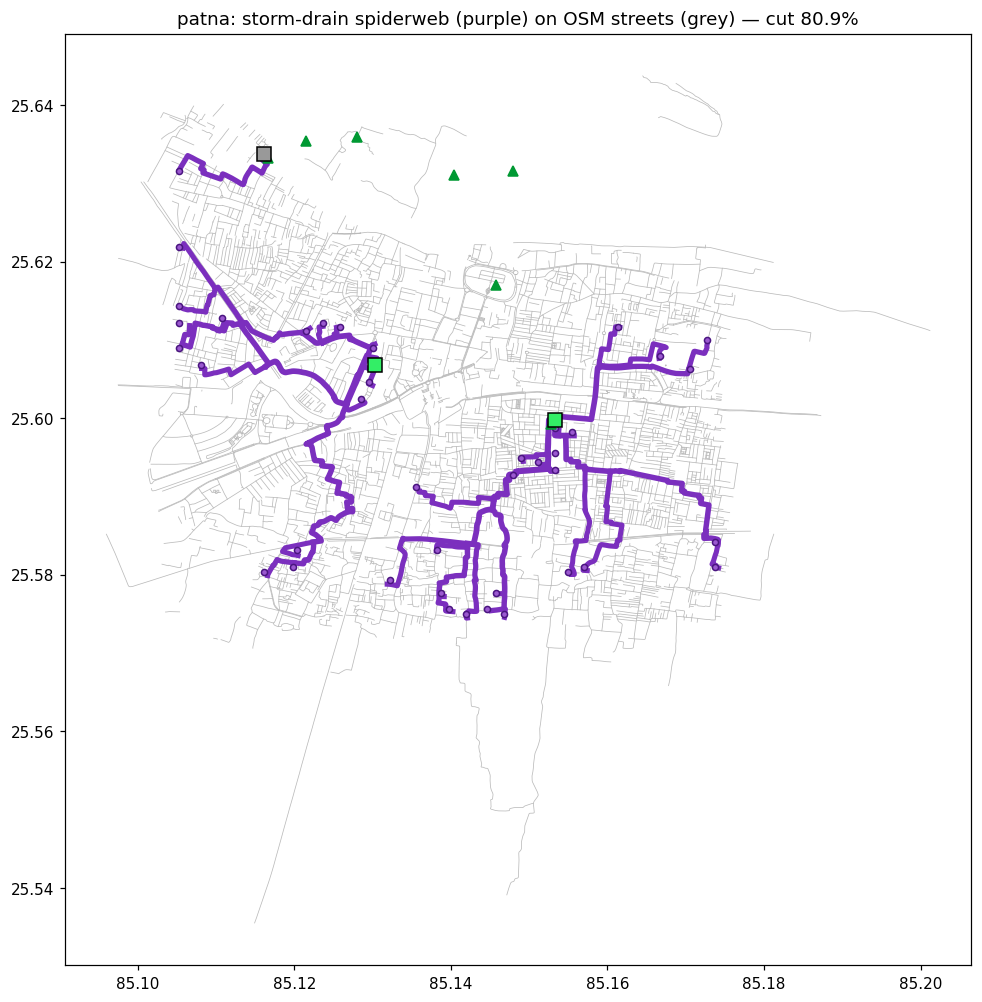
\includegraphics[width=.62\linewidth]{figures/spiderweb_patna.png}
\caption{The planned storm-drain spiderweb for Patna (purple; line width $\propto$ accumulated
flow) traces real OSM streets (grey) from 40 flood-basin inlets to detention pits and safe
low-ground outfalls. Measured cut: 80.9\% of street flooding at 100\,mm.}
\label{fig:web}
\end{figure}

\textbf{Results.} Across the four study areas the spiderweb cuts street flooding by 80.9\%
(Patna), 89.4\% (Patna-East), 80.3\% (Patna-West) and 72.6\% (Bengaluru), versus 21--26\% for the
sparse plans (Table~\ref{tab:ladder}, Figure~\ref{fig:web}); dose-response over 25--200\,mm is
monotone. Density improves \emph{economics} as well as efficacy: \rupee850/m$^3$ removed versus
\rupee1{,}309/m$^3$ for the sparse plan (Patna; Bengaluru \rupee1{,}121/m$^3$), because shared trunks
amortise length across basins. An adaptive storage planner provides the complementary curve --- each
micro-basin sized to its own gradient minimum; 727 sites buy a 30\% cut in Patna, while in
Bengaluru the stable part of the curve ends near 30\% (431 sites) and larger targets are honestly
reported as unreachable. The exposure layer grounds the maps in assets: at 100\,mm, 1{,}205 of
3{,}749 OSM buildings and 3{,}036 of 6{,}762 road segments in the Patna window are at risk.

\textbf{Why we believe these decisions despite \S\ref{sec:validation}.} The quantities that drive
the plans are the ones the ensemble shows to be robust: total flooded volume, basin existence and
approximate depth ordering, and downhill topology --- not the exact street that ponds first. The
planner's outputs are also \emph{portfolios} (many inlets, many micro-basins) whose value degrades
gracefully if any single pond shifts. We therefore frame outputs as relative planning guidance
(which strategy, what density, where first), not as certified absolute depths.

\section{Learned street-level risk, routing, and cross-city transfer}
\label{sec:gnn}
Both planning surfaces above route on graphs with hand-set costs: storm drains via a reverse
Dijkstra whose flow-direction cost ($\ell + 2400\,\Delta z^{+}$\,m) encodes a fixed uphill aversion,
and evacuation implicitly via raster overlays recomputed per storm. We replace the hand-set cost
with a learned one. \textbf{FloodGNN} is an edge-conditioned message-passing network
\citep{gilmer2017} (4 rounds, 96-dim states, $\sim$330k parameters, plain PyTorch) over the OSM
street graph (37{,}017 nodes / 79{,}928 directed edges for Patna), FiLM-conditioned on rainfall
\citep{perez2018film} so a single model covers the continuous storm range. Node features are
deliberately local and standardized per graph --- elevation anomaly, pit-ness, grade, flow
accumulation, permanent water, SAR waterlogging frequency, building/road density --- so nothing
identifies the city. Supervision is generated by the twin itself: the emulator's depth fields for a
20--240\,mm sweep sampled at street nodes and edges, and the drain planner's per-street conveyed
volume at three (rain, inlet-count) configurations ($\sim$9\,s of label generation per city, CPU).
Wet targets carry the same $\times$20 loss weight as the emulator (flooding is sparse;
\S\ref{sec:system}), validation holds out \emph{storm sizes} rather than nodes, and the shipped
checkpoint is the best-validation epoch.

FloodGNN answers three questions. \emph{Risk}: per-street flood depth at any rainfall in one
forward pass --- edge AUC \todo{TODO-COLAB} on held-out storms, vs 0.856 for a 24-epoch CPU smoke
model trained on Patna alone. \emph{Routing}: cost-inflated Dijkstra
($\ell \cdot (1 + 8\min(d,1.5) + 25\cdot[d>0.3\,\text{m}])$) yields evacuation routes crossing
\todo{TODO-COLAB}\,m of flooded street per route versus \todo{}\,m for the flood-ignorant shortest
path and \todo{}\,m for an oracle reading the emulator directly, at a \todo{}\% mean detour (150
random origin--destination pairs; the smoke model already recovers half the oracle's improvement:
$2{,}297 \to 1{,}735$\,m at $+24\%$ detour, oracle $1{,}172$\,m; Figure~\ref{fig:route}).
\emph{Placement}: the flow head reproduces the drain planner's trunk ranking (Spearman $\rho=$
\todo{TODO-COLAB}) without running it.

\textbf{Cross-city transfer.} Trained with Bengaluru held out entirely, FloodGNN ranks flooded
Bengaluru streets at AUC \todo{TODO-COLAB} zero-shot (reverse direction \todo{}), against \todo{}
when trained on all cities. A no-message-passing ablation (layers $=0$: the same features through a
per-node MLP) reaches only \todo{}, confirming that neighbourhood structure --- not raw local
topography --- carries the signal. This extends \S\ref{sec:validation} to learned models:
street-level flood knowledge is substantially city-transferable even where cell-level locations are
not, because message passing aggregates exactly the local basin context that single cells lack.

\textbf{Honesty and deployment.} FloodGNN distils the twin, so it inherits the twin's biases: its
claims are amortization, routing quality \emph{under} the twin's flood fields, and transfer --- not
the co-location skill that \S\ref{sec:validation} shows no topographic method has here.
(Supervising directly on SAR-observed street water is the natural next step.) The $\sim$1.3\,MB
checkpoint ships inside the dashboard image; \texttt{/api/route} answers from the GNN where present
and from the raster emulator otherwise, reporting its backend; a full-graph risk query takes
\todo{TODO-COLAB}\,ms on CPU versus \todo{}\,ms for the raster pipeline it amortizes.

\begin{figure}[t]
\centering
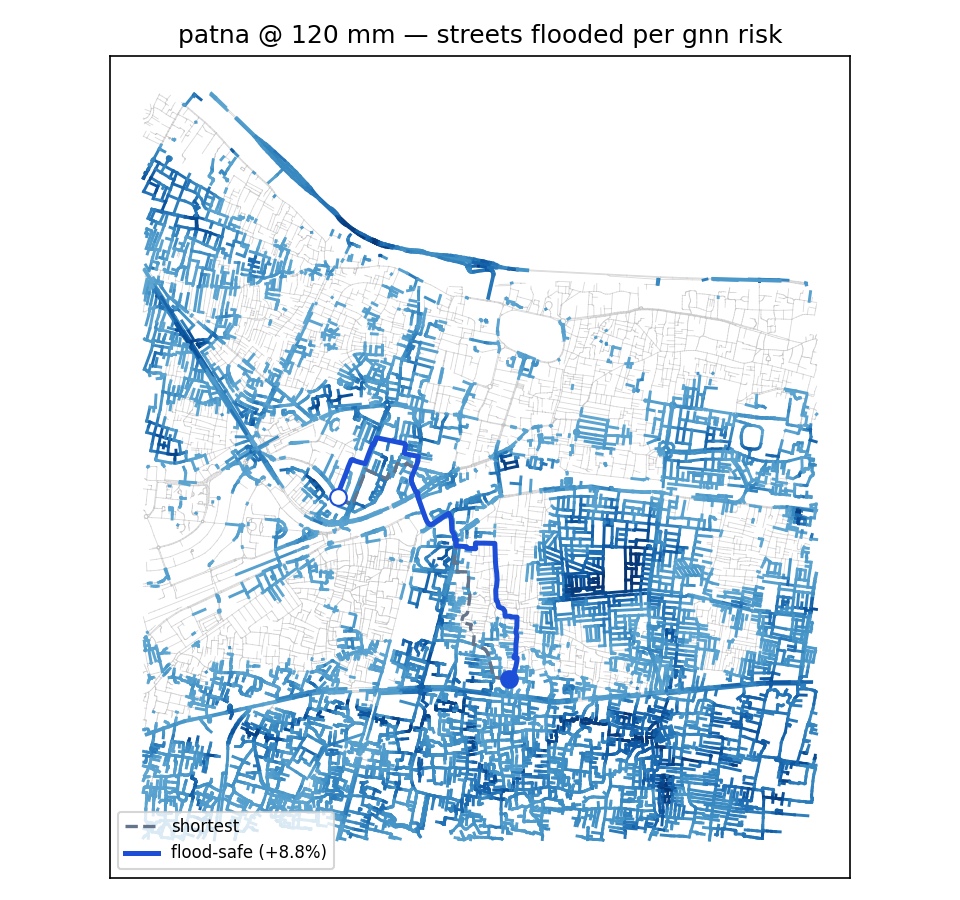
\includegraphics[width=.62\linewidth]{figures/route_demo_patna.png}
\caption{Flood-safe evacuation routing on the Patna street graph at 120\,mm: streets shaded by
GNN-predicted flood depth (blue = wet, grey = dry); the flood-ignorant shortest path (dashed)
versus the FloodGNN route (solid). The learned route trades a modest detour for crossing a
fraction of the floodwater --- live on the public dashboard at any rainfall.}
\label{fig:route}
\end{figure}

\section{Limitations and outlook}
Hydraulics run at 60\,m, coarser than the drawn street network; carved ``drains'' are full
60\,m cells, so absolute excavation volumes are resolution artifacts even though per-metre drain
costing is realistic. Depths are uncalibrated (and \S\ref{sec:validation} shows why per-class
physics calibration cannot fix co-location); groundwater recharge uses sample data pending CGWB
records. The natural next steps are finer national DEMs (e.g.\ CartoDEM), assimilating mapped
drain networks where they exist, sub-grid street conveyance, and validating the \emph{intervention
deltas} (not just state) against before/after SAR where cities have actually built drainage.

\section*{Reproducibility}
Code, per-city artifact bundles (including SAR masks and road graphs), tests, and runbooks:
\url{https://github.com/Maverick-Ansh/project-varuna}. Live dashboard:
\url{https://project-varuna-iota.vercel.app} (API: \texttt{anshvivek-varuna-floodtwin.hf.space}).
A new city builds with one script on a free Colab/Kaggle T4 and serves from the committed bundle.

\bibliographystyle{unsrtnat}
\bibliography{references}

\end{document}
